\input{../header.tex}

\subject{VERSUCH NUMMER 203}
\title{Verdampfungswärme und Dampfdruck-Kurve}
\date{
  Durchführung: DATUM
  \hspace{3em}
  Abgabe: DATUM
}

\begin{document}

\maketitle
\thispagestyle{empty}
\tableofcontents
\newpage
\setcounter{page}{1}
\section{Ziel}
\label{sec:Ziel}
\section{Theorie}
\label{sec:Theorie}

Der Doppler-Effekt beschreibt die Veränderung der Frequenz, wenn sich der Beobachter und eine Schallquelle relativ zu einander bewegen.
Bewegt sich die Quelle auf den Hörer zu, so wird die Grundfrequenz $\nu_0$ zu einer höheren Frequenz $\nu_{\text{gr}}$ verschoben.
Vergrößert sich der Abstand, reduziert sich die Frequenz zu $\nu_{\text{kl}}$.
Dabei gilt folgender mathematischer Zusammenhang
\begin{equation*}
    \nu_{\text{kl/gr}}=\frac{\nu_0}{1\mp \frac{v}{c}}\. .
\end{equation*}
Dieser Effekt wird in der Ultraschalltechnik verwendet, um z.B. die Geschwindigkeit von Blutströmungen zu ermitteln.
Wenn die Ultraschallwelle auf ein Blutkörper trifft, wird so die Frequenz $\nu_0$ verschoben.
Diese Verschiebung wird über die Formel
\begin{equation*}
    \Delta \nu=\nu_0 \frac{v}{c} (\cos{\alpha}+\cos{\beta}) 
\end{equation*}
beschrieben. Hierbei ist $v$ die Geschwindigkeit des Objektes, $c$ die Schallgeschwindigkeit und $\alpha$ und $\beta$ die Winkel zwischen Bewegungsrichtung und der 
Wellennormalen der ein- bzw. auslaufenden Welle.
\begin{figure}
    \centering
    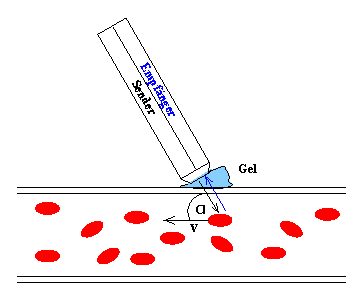
\includegraphics[width =6cm]{Blutstrom.pdf}
    \caption{Darstellung der Messung einer Blutstromgeschwingkeit mittels Doppler-Effekt\cite{apus3}.}
    \label{fig:Blutstrom}
\end{figure}
Da der Sender zugleich auch der Empfänger ist, sind die beiden Winkel $\alpha$ und $\beta$ identisch, sodass die Gleichung
\begin{equation}
    \Delta \nu=2\nu_0 \frac{v}{c} \cos{\alpha} 
    \label{eqn:dv}
\end{equation}
folgt.
Für den Dopplerwinkel folgt so 
\begin{equation}
    \alpha= 90° - \arcsin\left(\sin(\theta)\cdot\frac{c_\text{L}}{c_\text{P}}\right)\, .
    \label{eqn:alpha}
\end{equation}
Die Größen $c_\text{L}$ und $c_\text{P}$ sind hierbei die Schallgeschwindigkeiten in der Dopplerphantomflüssigkeit bzw. im Dopplerprisma.
Diese Messmethodik ist in \autoref{fig:Blutstrom} dargestellt.
Als Erzeuger und Empfänger der Ultraschallwellen dient ein Piezokristall.
Dieser Piezokristall wird einem elektrischen Wechselfeld ausgesetzt und dadurch zum Schwingen angeregt. Beim Schwingen emittiert der Kristall Ultraschallwellen.
\section{Aufbau}
\label{sec:Aufbau}

Die Messapparatur besteht aus einem Ultraschall Doppler-Generator im Pulsbetrieb sowie einer Ultraschallsonde mit einer Frequenz von $2\,\unit{\mega\hertz}$
und Untersuchungsobjekten. Die Ultraschallsonde dient dabei sowohl als Sender wie als Empfänger der Ultraschallwelle. 

Die Untersuchungsobjekte sind Strömungsrohre verschiedener Innen- und Außendurchmesser, welche mit einem Flüssigkeitsgemisch aus Wasser, Glycerin und 
Glaskugeln gefüllt ist. Die Strömungsgeschwindigkeit der Flüssigkeit wird im folgenden mit einer Zentrifugalpumpe eingestellt.

Um die Ankopplung der Ultraschallsonde an die Strömungsrohre zu erleichtern, werden Doppler-Prismen verwendet, die drei verschiedene Einfallswinkel besitzen, sodass 
der Winkel und der Abstand konstant gehalten werden kann. Die Dopplerprismen werden dabei auf das Rohrstücke gesetzt. Die Kontaktflächen werden mit einem Gel bedeckt, damit die Ultraschallwellen besser übertragen werden können.

\section{Durchführung}
\label{sec:Durchführung}

Der Versuch besteht aus zwei Teilversuchen. Zuerst wird die Strömungsgeschwindigkeit als Funktion des Dopplerwinkels $\Theta$ für fünf verschiedene
Flussgeschwindigkeiten gemessen. Dafür wird an der Zentrifugalpumpe eine Geschwindigkeit eingestellt; das Sample Volume des Ultraschallgenerators 
muss auf LARGE stehen. Nun werden mittels der Ultraschallsonde für jede Geschwindigkeit die Frequenzverschiebung $\symup{\Delta} \nu$ gemessen.

Im zweiten Versuchsteil wird das Strömungsprofil der Doppler-Flüssigkeit an einem 3/8-Schlauch mit einem Dopplerwinkel von 15° gemessen. Dazu muss zuerst 
das Sample Volume auf SMALL umgestellt werden. Mit dem Regler DEPTH lässt sich die Messtiefe einstellen. Bei einer maximalen Pumpleistung von 79\% 
wird die Strömungsgeschwindigkeit und der Streuintensitätswert gemessen. Begonnen bei einer Messtiefe von $30\,\unit{\milli\meter}$ bis zu einer 
Messtiefe von $11\,\unit{\milli\meter}$ werden die Werte in $0.75\,\unit{\milli\meter}$-Schritten aufgenommen. Die gesamte Messung wird für eine 
Pumpleistung von 45\% wiederholt.
\section{Auswertung}
\label{sec:Auswertung}

\subsection{Fehlerrechnung}
\label{sec:Fehlerrechnung}
Für die Fehlerrechnung werden folgende Formeln aus der Vorlesung verwendet.
für den Mittelwert gilt
\begin{equation}
    \overline{x}=\frac{1}{N}\sum_{i=1}^N x_i ß\; \;\text{mit der Anzahl N und den Messwerten x} 
    \label{eqn:Mittelwert}
\end{equation}
Der Fehler für den Mittelwert lässt sich gemäß
\begin{equation}
    \increment \overline{x}=\frac{1}{\sqrt{N}}\sqrt{\frac{1}{N-1}\sum_{i=1}^N(x_i-\overline{x})^2}
    \label{eqn:FehlerMittelwert}
\end{equation}
berechnen.
Wenn im weiteren Verlauf der Berechnung mit der fehlerhaften Größe gerechnet wird, kann der Fehler der folgenden Größe
mittels Gaußscher Fehlerfortpflanzung berechnet werden. Die Formel hierfür ist
\begin{equation}
    \increment f= \sqrt{\sum_{i=1}^N\left(\frac{\partial f}{\partial x_i}\right)^2\cdot(\increment x_i)^2}.
    \label{eqn:GaussMittelwert}
\end{equation}

Zunächst müssen die Dopplerwinkel $\alpha$ für die Winkel $\theta$ berechnet werden.
Die \autoref{eqn:alpha} liefert so 
\begin{align*}
     \alpha(\theta_{15}) &= 80.06\\
     \alpha(\theta_{30}) &=70.53\\
     \alpha(\theta_{45}) &=54.74\\
\end{align*}
\subsection{Bestimmung der Strömungsgeschwindigkeit}
\label{sec:Strömungsv}
Im ersten Teil der Auswertung wird die Strömungsgeschwindigkeit bestimmt. Die hierfür nötigen Messwerte sind in \autoref{tab:Stroemungsv} gelistet.
\begin{table}
    \centering
    \caption{Messwerte zu Bestimmung der Strömungsgeschwindigkeit.}
    \begin{tabular}{c c c c c c}
        \toprule
        Rpm der Pumpe  & Winkel $\theta \mathrm{/} \unit{\degree}$ & Winkel $\alpha \mathrm{/}  \unit{\degree}$ & $\nu_{\text{max}} \mathrm{/} \unit{\hertz}$ & $\nu_{\text{mean}} \mathrm{/} \unit{\hertz}$ &  $ \Delta\nu$ \\
        \midrule
        2990 & 15 & 80.06 & 175 & 85 & 90  \\
             & 30 & 70.53 & 210 & 110 & 100 \\
             & 60 & 54.74 & 303 & 159 & 144 \\
        4020 & 15 & 80.06 & 290 & 146 & 144 \\
             & 30 & 70.53 & 360 & 171 & 189 \\
             & 60 & 54.74 & 570 & 370 & 200 \\
        5010 & 15 & 80.06 & 380 & 183 & 197 \\
             & 30 & 70.53 & 565 & 269 & 296 \\
             & 60 & 54.74 & 960 & 513 & 447 \\
        6000 & 15 & 80.06 & 605 & 256 & 349 \\
             & 30 & 70.53 & 850 & 403 & 447 \\
             & 60 & 54.74 & 1505 & 757 & 748 \\
        7000 & 15 & 80.06 & 850 & 378 & 472  \\
             & 30 & 70.53 & 1160 & 519 & 641 \\
             & 60 & 54.74 & 2020 & 1013 & 1007 \\
        \bottomrule
    \end{tabular}
    \label{tab:Stroemungsv}
\end{table}
Eine Formel für dei Flussgeschwindigkeit ergibt sich durch das Umstellen von \autoref{eqn:dv} nach $v$
\begin{equation*}
v=\frac{c\cdot \Delta \nu}{2\nu_0\cdot \cos \alpha}\. .
\end{equation*}
So ergeben sich die folgenden Flussgeschwindigkeiten.
\begin{table}
     \centering
     \caption{Fließgeschwindigkeiten der verschiedenen Winkel und Pumpleistungen.}
     \begin{tabular}{c c c c c c}
          \toprule
          Rpm der Pumpe & $v_{15°}\mathrm{/} \unit{\frac{\meter}{\second}}$ & $v_{30°}\mathrm{/} \unit{\frac{\meter}{\second}}$& $v_{60°}\mathrm{/} \unit{\frac{\meter}{\second}}$ & $\bar{v}\mathrm{/} \unit{\frac{\meter}{\second}}$\\
          \midrule
          2990 & 0.2346 & 0.1350 & 0.1122 & 0.1605\\
          4020 & 0.3754 & 0.2552 & 0.1559 & 0.2621\\
          5010 & 0.5136 & 0.3996 & 0.3484 & 0.4205\\
          6000 & 0.9098 & 0.6035 & 0.5831 & 0.6988\\
          7000 & 1.2305 & 0.8654 & 0.7850 & 0.9603\\ 
          \bottomrule
     \end{tabular}
\end{table}
Neben der Berechnung der Geschwindigkeiten $v$ wird auch der Quotient der Frequenzverschiebung $\Delta \nu$ und der Kosinus des Dopplerwinkels $\alpha$ gegen die Geschwindigkeit $v$ aufgetragen.
Diese Graphen sind in \autoref{fig:Winkel15}, \autoref{fig:Winkel30} und \autoref{fig:Winkel45} dargestellt.
\begin{figure}
     \centering
     \includegraphics[height = 6cm]{build/plot11.pdf}
     \caption{Auftragung des Quotienten der Frequenzverschiebung $\Delta \nu$ und des Kosinus des Dopplerwinkels $\alpha=80.06$ gegen die Geschwindigkeit $v$.}
     \label{fig:Winkel15}
\end{figure}

\begin{figure}
     \centering
     \includegraphics[height = 6cm]{build/plot12.pdf}
     \caption{Auftragung des Quotienten der Frequenzverschiebung $\Delta \nu$ und des Kosinus des Dopplerwinkels $\alpha=70.53$ gegen die Geschwindigkeit $v$.}
     \label{fig:Winkel30}
\end{figure}

\begin{figure}
     \centering
     \includegraphics[height = 6cm]{build/plot13.pdf}
     \caption{Auftragung des Quotienten der Frequenzverschiebung $\Delta \nu$ und des Kosinus des Dopplerwinkels $\alpha=54.74$ gegen die Geschwindigkeit $v$.}
     \label{fig:Winkel45}
\end{figure}

Aufgrund der Tatsache, dass die Pumpe einen Defekt aufwies, welcher ein Anzeigen des Volumenstroms verhinderte, könne Theoretische Werte nur mit dem Abgleichen der maximalen Pumpleistung mit jener einer anderen Pumpe verglichen werden.
Die maximale Drehzahl der Pumpe waren $8700$ Rpm, der Volumenstrom der Vergleichspumpe liegt unter Volllast bei $7.5 \,\unit{\frac{\liter}{minute}}$. Mit der Querschnittsfläche des Rohrs von $0.025\, \unit{\centi \meter}^2$ kann so eine maximale Fließgeschwindigkeit von
$1.59 \, \unit{\frac{\meter}{\second}}$ angenommen werden.
Über den Dreisatz gilt es jetzt die Geschwindigkeiten für niedrigere Drehzahlen zu ermitteln.
Es ergeben sich folgende Werte 
\begin{align*}
     v_{7000\text{ Rpm}}&=1.2793\, \unit{\frac{\meter}{\second}}\\
     v_{6000\text{ Rpm}}&=1.0966\, \unit{\frac{\meter}{\second}}\\
     v_{5010\text{ Rpm}}&=0.9157\, \unit{\frac{\meter}{\second}}\\
     v_{4020\text{ Rpm}}&=0.7347\, \unit{\frac{\meter}{\second}}\\
     v_{2990\text{ Rpm}}&=0.5464\, \unit{\frac{\meter}{\second}}\, .\\
\end{align*}
\subsection{Bestimmung des Strömungsprofils}  
\label{sec:Profil}

Für den zweiten der Auswertung wird der Prismawinkel $\theta =30°$ verwendet. Die gemessenen Geschwindigkeiten und Streuintensität für 2 Pumpdrehzahlen sind in \autoref{tab:3920rpm} und \autoref{tab:6100rpm} aufgetragen.
Darunter sind die Geschwindigkeiten und Streuintensitäten der Drehzahlen je gegen die MEsstiefe aufgetragen.
 \begin{table}
     \centering
     \caption{Streuintensität und Geschwindigkeit bei 3920 Umdrehungen pro Minute.}
     \begin{tabular}{c c c c c}
         \toprule
         Messtiefe $ \mathrm{/} \unit{\micro \second}$ &  Messtiefe $ \mathrm{/} \unit{\milli \meter}$ & $v \mathrm{/} \unit{\frac{\centi \meter}{\second}}$ & $v \mathrm{/} \unit{\frac{\meter}{\second}}$ & $I \mathrm{/} 1000\unit{\frac{V^2}{\second}}$\\
         \midrule
         12.0 &  -0.42 &  13.2 &  0.132 &  460\\
         12.5 &  0.33 &  11.5 &  0.115 &  1160\\
         13.0 &  1.08 &  13.2 &  0.132 &  1500\\
         13.5 &  1.83 &  14.8 &  0.148 &  1200\\
         14.0 &  2.58 &  14.8 &  0.148 &  1000\\
         14.5 &  3.33 &  16.5 &  0.165 &  1000\\
         15.0 &  4.08 &  16.5 &  0.165 &  1500\\
         15.5 &  4.83 &  16.5 &  0.165 &  1650\\
         16.0 &  5.58 &  16.5 &  0.165 &  1900\\
         16.5 &  6.33 &  16.5 &  0.165 &  1200\\
         17.0 &  7.08 &  16.5 &  0.165 &  750\\
         17.5 &  7.83 &  16.5 &  0.165 &  400\\
         18.0 &  8.58 &  16.5 &  0.165 &  350\\
         18.5 &  9.33 &  16.5 &  0.165 &  340\\
         19.0 &  10.08 &  14.8 &  0.148 &  320\\
         19.5 &  10.83 &  14.8 &  0.148 &  310\\
         \bottomrule
     \end{tabular}
     \label{tab:3920rpm}
\end{table}
\begin{table}
     \centering
     \caption{Streuintensität und Geschwindigkeit bei 6100 Umdrehungen pro Minute.}
     \begin{tabular}{c c c c c}
          \toprule
          Messtiefe $ \mathrm{/} \unit{\micro \second}$ &  Messtiefe $ \mathrm{/} \unit{\milli \meter}$ & $v \mathrm{/} \unit{\frac{\centi \meter}{\second}}$ & $v \mathrm{/} \unit{\frac{\meter}{\second}}$ & $I \mathrm{/} 1000\unit{\frac{V^2}{\second}}$\\
          \midrule
          12.0 &  -0.42 &  38.2 &  0.382 &  800\\
          12.5 &  0.33 &  44.6 &  0.446 &  1700\\
          13.0 &  1.08 &  50.9 &  0.509 &  2600\\
          13.5 &  1.83 &  57.3 &  0.573 &  3500\\
          14.0 &  2.58 &  66.8 &  0.668 &  3500\\
          14.5 &  3.33 &  76.4 &  0.764 &  3000\\
          15.0 &  4.08 &  82.7 &  0.827 &  2700\\
          15.5 &  4.83 &  82.7 &  0.827 &  2400\\
          16.0 &  5.58 &  82.7 &  0.827 &  2100\\
          16.5 &  6.33 &  73.2 &  0.732 &  1800\\
          17.0 &  7.08 &  70.0 &  0.700 &  1400\\
          17.5 &  7.83 &  66.8 &  0.668 &  1200\\
          18.0 &  8.58 &  66.8 &  0.668 &  1200\\
          18.5 &  9.33 &  66.8 &  0.668 &  1150\\
          19.0 &  10.08 &  70.0 &  0.700 &  1000\\
          19.5 &  10.83 &  73.2 &  0.732 &  800\\
          \bottomrule
     \end{tabular}
     \label{tab:6100rpm}
\end{table}

Der Nullpunkt der Messtiefe liegt hierbei auf der Oberfläche des Rohres.


\begin{figure}
     \centering
     \includegraphics[height = 6cm]{build/rpm39201.pdf}
     \caption{Geschwindigkeit aufgetragen gegen die Messtiefe bei 3920 Rpm.}
     \label{fig:39201}
\end{figure}

\begin{figure}
     \centering
     \includegraphics[height = 6cm]{build/rpm39202.pdf}
     \caption{Strömungsintensität aufgetragen gegen die Messtiefe bei 3920 Rpm.}
     \label{fig:39202}
\end{figure}

\begin{figure}
     \centering
     \includegraphics[height = 6cm]{build/rpm61001.pdf}
     \caption{Geschwindigkeit aufgetragen gegen die Messtiefe bei 6100 Rpm.}
     \label{fig:61001}
\end{figure}

\begin{figure}
     \centering
     \includegraphics[height = 6cm]{build/rpm61002.pdf}
     \caption{Strömungsintensität aufgetragen gegen die Messtiefe bei 6100 Rpm.}
     \label{fig:61002}
\end{figure}
\section{Diskussion}
\label{sec:Diskussion}

In \autoref{sec:Strömungsv} ist der zu erwartende lineare Zusammenhang von $\frac{\Delta \nu}{\cos \alpha}$ mit der Strömungsgeschwindigkeit $v$. Ein Vergleich zu einem Theoriewert bleibt jedoch aus, 
da aufgrund eines technischen Defekts die Durchflussrate der Pumpe nicht angezeigt werden konnte. Den Graphen ist jedoch zu entnehmen, dass trotz der Verwackelungen, die durch das Halten der Sonde entstanden ist, und 
der Tatsache, dass sich die Drehzahl der Pumpe nach einer Weile automatisch erhöht hat, die Messwerte relativ frei von Messungenauigkeiten sind. DIe Messwerte liegen alle auf der jeweiligen Ausgleichsgeraden.

In \autoref{sec:Profil} wird das Strömungsverhalten untersucht. Es war zu erwarten, dass sowohl die Strömungsgeschwindigkeit als auch die -intensität zunimmt, je weiter die Messtiefe in die Röhre eindringt.
Nach erreichen des Mittelpunktes ist zu erwarten, dass beide Messgrößen wieder abnehmen. Im Groben zeichnet sich auch dieser Trend bei den Messwerten ab. Jede der Kurven hat einen Peak bei bei einer im Rohr liegenden Messtiefe, welcher jedoch nicht ganz bei dem zu erwartenden Wert liegt.
Da das Rohr einen Außendurchmesser von $15\,$mm und einen Innendurchmesser von $10\,$ mm, ist der nach der Eichung zu erwartende Peak bei einer Messtiefe von $7.5\,$mm


\newpage
\printbibliography
\nocite{ap308}
\nocite{matplotlib}
\nocite{numpy}
\nocite{scipy}
\nocite{uncertainties}
\nocite{reback2020pandas}

\newpage
%\includepdf[scale=0.9,pages=1,pagecommand=\section*{Anhang}\thispagestyle{empty}]{messdaten.pdf}
%\addcontentsline{toc}{section}{\protect\numberline{}Anhang}
%\includepdf[scale=0.9,pages=2-]{messdaten.pdf}
%\includepdf[pages=-]{messdaten.pdf}

\end{document}
